\chapter{Resultados de TDA sobre trayectorias} \label{chp:resultados}
En este capítulo se presentan los resultados obtenidos a lo largo del análisis topológico de trayectorias utilizando técnicas de TDA, junto con algunos enfoques comparativos mediante métodos clásicos de análisis de datos. El objetivo principal de esta sección es mostrar de forma clara y estructurada cómo las herramientas aplicadas permiten extraer información significativa sobre la estructura de los datos, tanto a nivel local como global.

\vspace{0.2cm}

Se incluyen visualizaciones de nubes de puntos generadas a partir de trayectorias GPS del conjunto Geolife, así como sus correspondientes diagramas de persistencia, representaciones PCA y grafos Mapper. También se analizan las propiedades topológicas identificadas —como ciclos persistentes o conectividad— y se discuten sus implicaciones. Adicionalmente, se presentan resultados de métodos alternativos no topológicos (como clustering y reducción de dimensionalidad) con el fin de establecer una comparación cualitativa entre enfoques.

\vspace{0.2cm}

La interpretación de los resultados se centra tanto en trayectorias individuales como en el comportamiento agregado del conjunto de datos, permitiendo evaluar la capacidad del TDA para detectar patrones globales, anomalías y propiedades invariantes que no son fácilmente identificables mediante técnicas convencionales.


\section{Resultados} \label{sct:resultados_resultados}

Durante este capítulo, se van a plantear los resultados del análisis topológico de datos explicada a lo largo del capítulo \ref{chp:desarrollo} sobre una sola trayectoria del dataset \textit{Geolife}, sobre un conjunto de trayectorias consecutiva del mismo, y sobre otro conjunto de trayectorias no relacionadas entre sí, así como la aplicación de estos mismos datos en su contraparte implementada con métodos tradicionales. Posteriormente, se presentarán las características topológicas observadas a lo largo del desarrollo, y se hará una breve comparativa entre las 2 soluciones, y se intentará dar una visión a las diferencias entre los resultados en la ejecución de las mismas.

\vspace{2cm}
En primer lugar, vamos a observar el resultado de aplicar estos análisis a una sola trayectoria del conjunto \textit{Geolife}. Como se ha visto anteriormente en el capítulo \ref{chp:desarrollo}, en primer lugar se realizó una visualización de mapa de puntos en 3 dimensiones de la trayectoria en sí. 

Se observa en este caso que al ser una trayectoria de puntos consecutivos, se ve una linea bien definida en su movimiento, pudiendo deducirse que produjo un desplazamiento mayormente vertical en primera, seguido de una serie de desplazamientos horizontales que podrían asimilar la toma de una curva.

\begin{figure}[H]
    \centering
    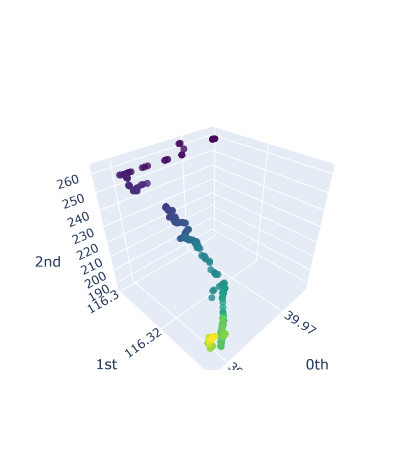
\includegraphics[scale=0.5]{images/puntos_trayec_sola.png}
    \caption{Nube de puntos de una Trayectoria}
    \label{fig:sola_trayec_nube}
\end{figure}

Esta visualización nos ofrece una primera idea de las características topológicas que podría tener esta trayectoria. En general, la visualización 3D no es eficaz, al ser compleja, y no es compatible con trayectorias de mayor dimensión. Para poder obtener resultados, debemos aplicar las herramientas mencionadas anteriormente, como seria la generación del diagrama de persistencia \ref{fig:pers_una} y el grafo Mapper \ref{fig:grafo_mapper}, así como la matriz de distancia entre los puntos de la trayectoria \ref{fig:matriz}. 

\begin{figure}[htbp]
    \centering
    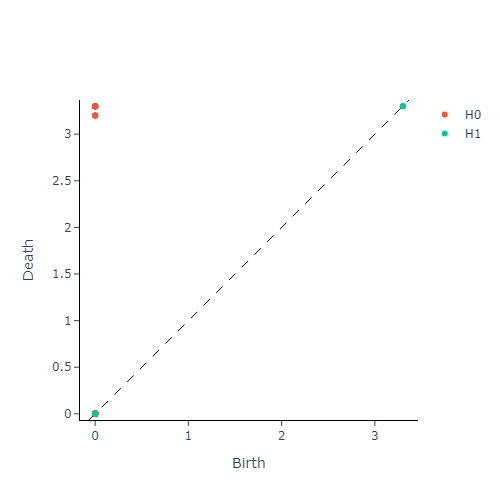
\includegraphics[width=0.7\linewidth]{images/persistencia_una.png}
    \caption{Diagrama de Persistencia de una trayectoria }
    \label{fig:pers_una}
\end{figure}

\begin{figure}[htbp]
    \centering
    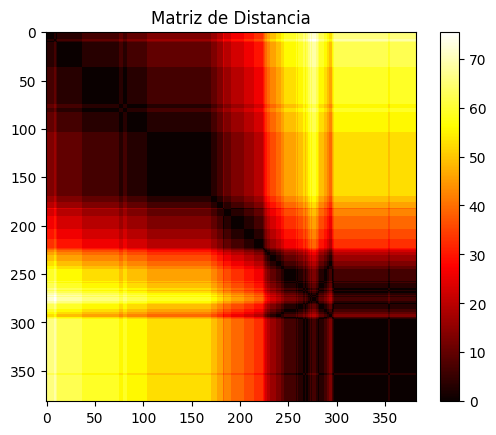
\includegraphics[scale=0.75]{images/matriz.png}
    \caption{Matriz de Distancia de los puntos de la trayectoria}
    \label{fig:matriz}
\end{figure}

\begin{figure}[htbp]
    \centering
    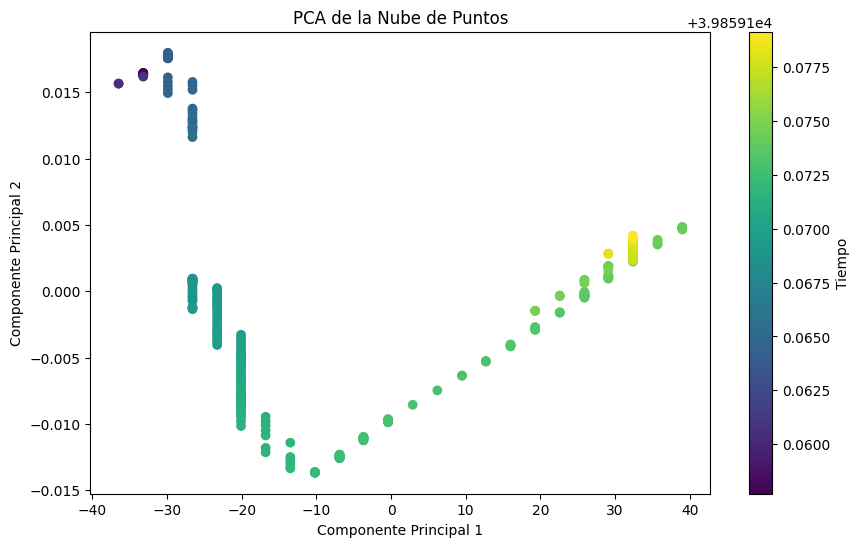
\includegraphics[width=0.75\linewidth]{images/pca_una.png}
    \caption{Análisis con PCA}
    \label{fig:enter-label}
\end{figure}

A partir de estos tres componentes del análisis, podemos afirmar una serie de hechos sobre la naturaleza de esta trayectoria. En primer lugar, 
la visualización en tres dimensiones ( Figura \ref{fig:sola_trayec_nube} ) nos indica que la trayectoria es continua en el espacio, sin cambios abruptos en altitud ni desplazamientos bruscos en el plano horizontal. Este comportamiento sugiere que el movimiento del agente fue progresivo y suave, lo que es coherente con trayectorias humanas o de vehículos en contextos urbanos o semiurbanos.

En segundo lugar, el análisis topológico de la trayectoria mediante homología persistente (Figura~\ref{fig:pers_una}) confirma que la trayectoria se comporta como una única componente conexa (grupo de homología \(H_0\)), ya que todos los puntos rojos aparecen cerca del origen y mueren rápidamente. Esto indica que no hay trayectos desconectados ni segmentos aislados dentro del recorrido.

Por otro lado, la presencia de un ciclo detectado en la dimensión uno (\(H_1\)), representado por un punto verde alejado de la diagonal, revela una característica topológica significativa: la trayectoria contiene una curva cerrada o un bucle. Esta información sería difícil de detectar a simple vista, y gracias al enfoque topológico, puede interpretarse como una posible zona de retorno, giro o patrón de navegación circular realizado por el agente.

Finalmente, la ausencia de características en dimensión dos (\(H_2\)) corrobora que no existen cavidades tridimensionales cerradas dentro del conjunto de puntos, lo cual es esperable dado que el movimiento ocurre sobre una superficie terrestre y no en un volumen tridimensional cerrado.

Además del análisis topológico, se aplicó una reducción de dimensionalidad utilizando Análisis de Componentes Principales (PCA) con el objetivo de visualizar la trayectoria en un espacio bidimensional conservando la mayor varianza posible de los datos originales. En este análisis, se observó cómo la trayectoria proyectada mantiene una estructura coherente, lo que valida que la geometría global del recorrido puede conservarse parcialmente incluso al reducir la dimensionalidad. No obstante, a diferencia del análisis topológico, el PCA no es capaz de identificar la presencia de bucles o estructuras conexas, ya que estas propiedades no se manifiestan directamente en la varianza lineal de los datos.

En este apartado, vamos a observar el resultado de aplicar herramientas topológicas a un \textbf{conjunto de trayectorias}, utilizando el framework desarrollado y descrito en el capítulo \ref{chp:desarrollo}. Para ello, se aplicaron técnicas de Análisis Topológico de Datos (TDA), comenzando con la construcción del grafo Mapper, el cálculo de la homología persistente y la proyección mediante Análisis de Componentes Principales (PCA).

\begin{figure}[htbp]
    \centering
    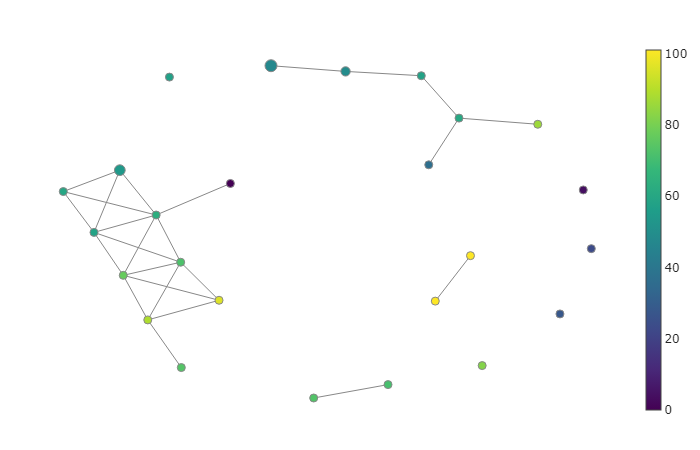
\includegraphics[width=0.75\linewidth]{images/MAPPER_VARIAS.PNG}
    \caption{Grafo Mapper de múltiples trayectorias}
    \label{fig:grafo_mapper_varias}
\end{figure}

En la Figura \ref{fig:grafo_mapper_varias}, se presenta el resultado del algoritmo Mapper aplicado al conjunto completo. Esta visualización revela una estructura compuesta por varias componentes conectadas y otras aisladas. Se puede observar una componente densa (a la izquierda del grafo), que agrupa trayectorias con características similares, mientras que otros nodos aislados indican trayectorias con comportamientos significativamente distintos. La coloración de los nodos representa algún valor escalar asignado, como una función de filtro (por ejemplo, centralidad o densidad), lo que permite identificar posibles agrupamientos o trayectorias atípicas.

\begin{figure}[htbp]
    \centering
    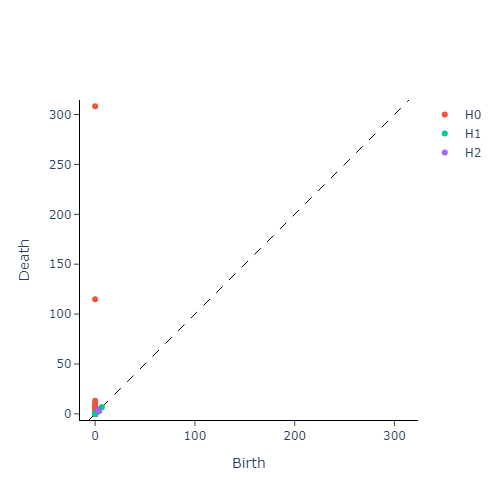
\includegraphics[width=0.7\linewidth]{images/persistencia.png}
    \caption{Diagrama de Persistencia para el conjunto de trayectorias}
    \label{fig:pers_varias}
\end{figure}

La Figura \ref{fig:pers_varias} muestra el diagrama de persistencia del conjunto, el cual permite analizar las características topológicas de las trayectorias en distintas dimensiones. En el módulo de homología cero ($H_0$), correspondiente a componentes conexas, observamos un gran número de puntos que nacen y mueren rápidamente, lo cual sugiere que muchas trayectorias comienzan como componentes aisladas que se conectan gradualmente. Algunos puntos rojos más lejanos de la diagonal indican componentes que persisten más tiempo, es decir, trayectorias bien definidas y separadas del resto.

En el módulo de homología ($H_1$), representada por los puntos verdes, se observa la presencia de varios ciclos, algunos de los cuales son persistentes. Esto indica que dentro del conjunto existen trayectorias que forman bucles o retornos. Estas estructuras topológicas son relevantes, ya que pueden estar relacionadas con patrones de desplazamiento cíclico, como recorridos circulares, vueltas o trayectorias repetitivas en ciertos espacios.

Se detecta un solitario punto en módulo de homología ($H_2$), siendo este punto una anomalía entre los valores de las trayectorias, posiblemente un error a la hora de medir los datos en alguno de los instantes tomados, ya que al representar las trayectorias movimientos sobre superficies planas o cuasi-planas (como mapas urbanos) y no en espacios tridimensionales cerrados, no debería haber cavidades dentro de este conjunto consecutivo de trayectorias. Al revisar los datos, se observa que efectivamente un error en los valores de una de las 110 trayectorias leídas es el causante de este punto. Este valor habría sido casi imposible de detectar sin hacer uso de este tipo de métodos.

\begin{figure}[htbp]
    \centering
    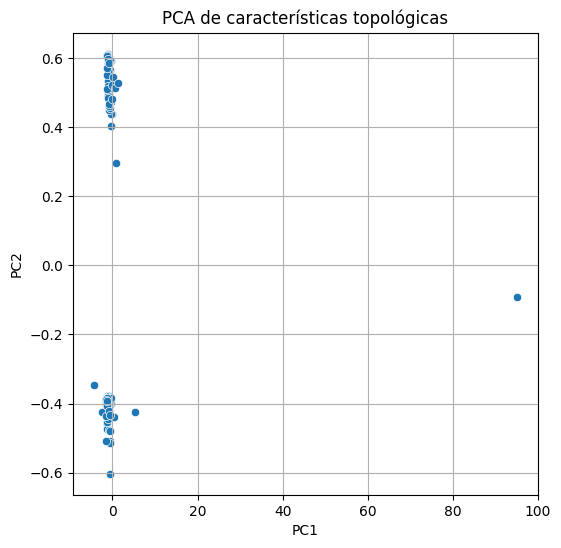
\includegraphics[width=0.75\linewidth]{images/pca_varias.png}
    \caption{Análisis PCA de características topológicas}
    \label{fig:pca_varias}
\end{figure}

En la Figura \ref{fig:pca_varias}, se presenta la proyección de las trayectorias en un espacio de dos dimensiones mediante PCA. Esta técnica se aplicó a los vectores de características topológicas derivados (como la persistencia en $H_0$, $H_1$, entre otros). La mayoría de los puntos se agrupan en una región cercana al eje vertical, lo cual indica que comparten una estructura topológica similar. Sin embargo, destaca un punto que se aleja notablemente en el eje $PC1$, lo que sugiere la presencia de una trayectoria con una topología significativamente diferente al resto. Esta trayectoria podría corresponder a un \textit{outlier}, detectado gracias al poder de discriminación del análisis topológico.

\vspace{0.4cm}

En conjunto, estos tres componentes del análisis nos permiten concluir que el conjunto de trayectorias analizado presenta una variedad rica de estructuras topológicas. Existen trayectorias que forman patrones recurrentes (loops), algunas con comportamiento similar agrupadas en clústeres, y otras más atípicas o anómalas. Herramientas como Mapper, homología persistente y PCA permiten explorar estos datos más allá de su geometría directa, capturando propiedades de conectividad, ciclos y diversidad estructural.

\subsection{Análisis de clustering y comparación con métodos de TDA}

Además del análisis topológico previamente presentado, se exploraron otros métodos más tradicionales para el análisis de las trayectorias, con el fin de contrastar sus resultados y comprender mejor la naturaleza del conjunto de datos. Para ello, se aplicaron técnicas de agrupamiento como DBSCAN y KMeans, así como un Análisis de Componentes Principales (PCA) clásico sobre todas las trayectorias reducidas. 

En primer lugar, en la Figura~\ref{fig:tsne_cluster} se presentan los resultados de la reducción de dimensionalidad mediante t-SNE, sobre la cual se aplicaron los algoritmos de agrupamiento DBSCAN y KMeans.

\begin{figure}[htbp]
    \centering
    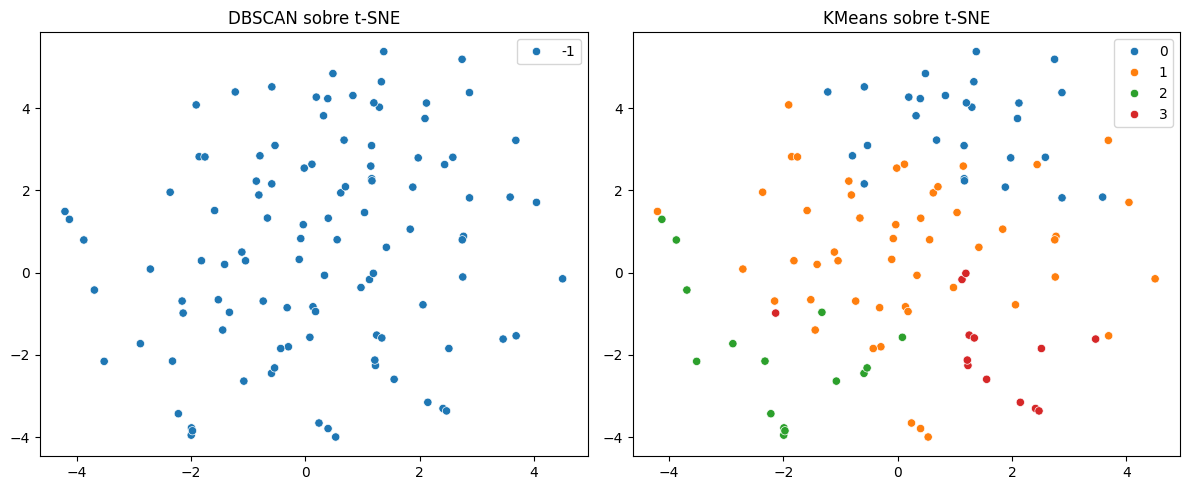
\includegraphics[width=\linewidth]{images/dbscan_kmeans.png}
    \caption{Resultados de clustering sobre reducción t-SNE: DBSCAN (izquierda) y KMeans (derecha)}
    \label{fig:tsne_cluster}
\end{figure}

En el caso de DBSCAN, se observa que el algoritmo no logra identificar estructuras claras de agrupamiento, asignando a todos los puntos la misma etiqueta (o marcándolos como ruido). Esto sugiere que las trayectorias no presentan densidades locales suficientemente diferenciadas para que DBSCAN pueda formar clústeres robustos, o que los parámetros utilizados no eran adecuados para la distribución de los datos en este espacio reducido. Este comportamiento contrasta con los resultados del análisis topológico, donde se identificaban componentes conectadas y ciclos, lo cual indica que sí existe una estructura no trivial en los datos que DBSCAN no ha podido capturar.

Por otro lado, el método KMeans sí fue capaz de dividir el conjunto en cuatro clústeres distintos. Estos grupos parecen estar distribuidos con cierta coherencia espacial, aunque el método se basa únicamente en distancias euclidianas en el espacio reducido por t-SNE. Sin embargo, KMeans no puede detectar bucles o estructuras de conectividad, lo cual representa una limitación frente al análisis de homología persistente. A pesar de ello, los resultados de KMeans pueden ser útiles para la clasificación general de patrones de trayectorias en función de su forma proyectada.

También se realizó un Análisis de Componentes Principales (PCA) tradicional sobre el conjunto de trayectorias para visualizar la distribución global de las mismas en un espacio linealmente reducido (Figura~\ref{fig:pca_tradicional}).

\begin{figure}[htbp]
    \centering
    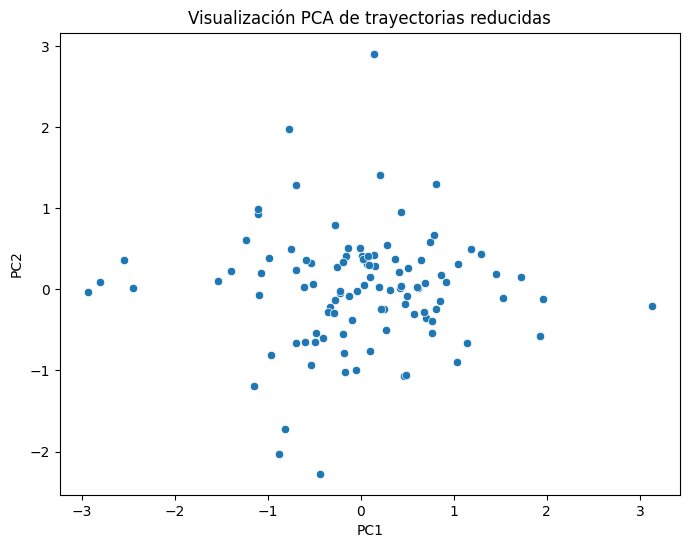
\includegraphics[width=0.75\linewidth]{images/PCA_tradicional.png}
    \caption{PCA tradicional sobre trayectorias}
    \label{fig:pca_tradicional}
\end{figure}

En esta representación, se aprecia una nube de puntos concentrada cerca del origen, con algunas trayectorias dispersas hacia los extremos. Esto indica una cierta homogeneidad en el comportamiento general de las trayectorias, con algunas excepciones que podrían representar trayectos atípicos. No obstante, al igual que en el PCA aplicado a características topológicas, esta visualización no permite identificar características como ciclos o componentes desconectadas, las cuales son evidenciadas únicamente a través del análisis topológico.

\bigskip

\textbf{Comparación con métodos topológicos:}

\begin{itemize}
    \item \textbf{PCA y t-SNE:} Ambos métodos de reducción de dimensionalidad son útiles para representar visualmente la distribución de trayectorias, pero no capturan propiedades topológicas como la conectividad o la existencia de ciclos. Esto limita su capacidad para detectar patrones más complejos de movimiento.
    
    \item \textbf{DBSCAN y KMeans:} Estos algoritmos permiten segmentar los datos en grupos, pero dependen fuertemente de la métrica y del espacio de representación. En especial, DBSCAN no resultó efectivo en este contexto. KMeans, aunque más útil, tampoco proporciona información sobre la estructura topológica de las trayectorias.
    \item \textbf{Homología Persistente y Mapper:} En comparación, el análisis topológico ofrece una visión más rica del comportamiento de las trayectorias. Permite detectar bucles, componentes conexas y variaciones estructurales que los métodos convencionales no logran identificar.
\end{itemize}

En conclusión, los métodos clásicos como PCA, t-SNE y clustering son complementarios al análisis topológico. Mientras los primeros proporcionan una visión global basada en distancias y varianza, el segundo aporta información clave sobre la forma y conectividad de las trayectorias, siendo particularmente útil para identificar patrones complejos de movimiento.



%%%%%%%%%%%%%%%%%%%%%%%%%%%%%%%%%%%%%%%%%%%%%%%%%%%%%%%%%%%%%%%%%%%%%%%%%%%%%%%%
%%%%%%%%%%%%%%%%%%%%%%%%%%%%%%%%%%%%%%%%%%%%%%%%%%%%%%%%%%%%%%%%%%%%%%%%%%%%%%%%









